\documentclass[11pt]{amsart}

% Standard letter size paper with 1inch margins
\usepackage[letterpaper, margin=1in]{geometry}
\usepackage{float}
% Useful packages 
\usepackage{amsmath, amssymb, amsthm, amsaddr}
\usepackage{enumerate, subcaption, graphicx, hyperref}
\usepackage{xcolor}
\usepackage{diagbox}



\title{AMATH 482/582: Homework 4}
\author{Sathvik Chinta} % first and last name

\date{\today} % you can also just type the date instead of "\today"

\begin{document}

\maketitle 

\begin{abstract}
     
    % Your report should contain a brief, 100 word abstract describing what is contained in 
    % the document and what you did. {\bf Don't forget 6 pages max}.
\end{abstract}


\section{Introduction and Overview}\label{sec:Introduction}

% Here you will give a brief introduction to the problem you solved. Including 
% some discussion of relevant literature and background. 

% Make sure you use the correct citation commands (i.e., \texttt{$\backslash$cite}) to keys 
% from your bib file like this \cite{example-article-citation}. If you want 
% to cite more than one reference simply use \cite{example-article-citation, example-book-citation}. You can grab latex citations 
% from \href{https://scholar.google.com}{Google Scholar}. Just keep in mind that they often 
% need to be cleaned up.

\section{Theoretical Background}\label{sec:theory}

We will use spectral clustering in the beginning to see 
if we can get reliable results. Spectral clustering is a
method for deeply rooted in graph theory. In our case, each of the 
data points would get treated as a node in our graph. In order to perform spectral clustering, 
we will use a Laplacian matrix on our set of points. A laplacian matrix can be defined as 

\begin{equation*}
    L_{i,j} = 
    \begin{cases}
      \text{deg}(v_i) \text{ if } i = j\\      
      -1 \text{ if } i \neq j \text{ and } v_i \text{ is adjacent to } v_j\\
      0 \text{ otherwise }
    \end{cases}
\end{equation*}

Equivalently, we can define two matrices: the degree matrix (D) and the adjacency matrix (A) and define the laplacian 
matrix with the equation:

\[L = D - A\]

We can then check the closely connected nodes which, in theory, should be 
closely related to each other as well. The components of the eigenvectors that correspond 
to the smallest eigenvalues of our constructed laplacian matrix, then, can be used 
to find clusters in our graph. 

The second eigenvalue of the laplacian matrix is called the Fiedler value. The magnitude of this 
reflects how connected the graph is as a whole. We can select the Fiedler vector (the second eigenvector)
and use the components whose value is positive to signify us predicting the +1 case (either democrat or republican)
and the value who is negative to signify us predicting the -1 case (the other party).
% You dedicate this section to the theoretical background of the methods and frameworks 
% that you used in your homework. This is not meant to reproduce material from the lectures
%  or references you used but rather to demonstrate your understanding of the 
%  mathematical foundations of the methods and algorithms. You can create equations like this 
%  \begin{equation*}
%      f(x) = \int_A \sin( \pi x) dx.
%  \end{equation*}
%  You do not need to label your equations unless they are referenced in the text. In that 
%  case simply use 
%  \begin{equation}\label{eq:meaningful-label}
%       - \frac{\partial^2 u}{\partial x^2} = \sin ( \pi x).
%  \end{equation}
% Also look up the \texttt{align} or \texttt{aligned} environments if you want multi-line 
% equations. You can then reference your equations in text using the $\backslash$\texttt{eqref}
% command as such \eqref{eq:meaningful-label}. 

\section{Algorithm Implementation and Development}\label{sec:algorithms}


% Here you discuss the algorithms and software packages that you used. Not much to it. 
% Just make sure you cite the packages properly and avoid including code. 
% You are welcome to use \LaTeX packages that are specifically designed to show 
% algorithms such \href{https://www.overleaf.com/learn/latex/Algorithms}{as this}, but it is 
% not always worth the effort and real estate. 


\section{Computational Results}\label{sec:results}
Plotting the sigma values (1000 values between 0 and 4) against accuracy for spectral clustering yields the following plot: 
\begin{figure}[H]
    \centering
    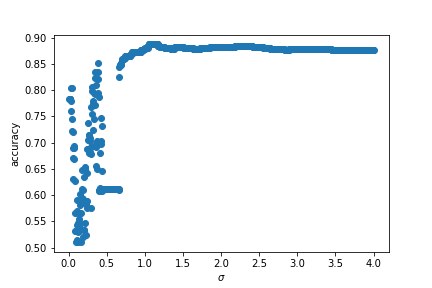
\includegraphics[width=0.8\textwidth]{/home/sathvikc/AMATH-482-2/AMATH-482/Homework Assignments/Homework 4/sigma_accuracy.png}
    \caption{Plot of sigma values against accuracy for spectral clustering}
    \label{fig:sigma_accuracy}
\end{figure}

We can see that the accuracy of the spectral clustering increases drastically after about $\sigma = 0.75$. 
Until that point, the accuracy seems to fall drastically at the smaller sigma values, then increase as well. 
After $\sigma = 0.75$, the accuracy seems to stabilize in the high 0.8's. The maximum accuracy occurs when $\sigma = 1.\overline{053}$. The accuracy at this point is 
0.887, which indicates that even though our spectral clustering seems to be unstable, we are still getting 
a good accuracy. 

When using the semi-supervised learning technique, we get the following results for different 
values of M and J.

\begin{tabular}{|c|ccccc|}
     \hline
     \diagbox{J}{M} & 2 & 3 & 4 & 5 & 6 \\
     \hline
        5  & 0.8827 & 0.8827 & 0.8620 & 0.8827 & 0.8827\\
        10 & 0.8781 & 0.8919 & 0.8873 & 0.8873 & 0.8160\\
        20 & 0.8850 & 0.8873 & 0.8988 & 0.8735 & \color{red}0.7816\\
        40 & 0.8850 & 0.8942 & 0.9011 & 0.9264 & \color{green}0.9310\\
     \hline
\end{tabular}

\begin{figure}[H]
    \centering
    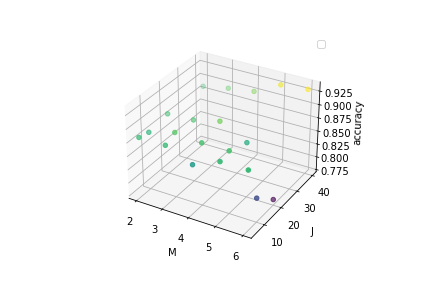
\includegraphics[width=0.8\textwidth]{/home/sathvikc/AMATH-482-2/AMATH-482/Homework Assignments/Homework 4/M_J_accuracyFewPoints.png}
    \caption{Plot of M and J values against accuracy for semi-supervised learning}
    \label{fig:M_J_accuracyFew}
\end{figure}

We can see that the accuracy of the semi-supervised learning algorithm is almost as good, if not better, than
that of the spectral clustering algorithm in most cases. The best accuracy occurs when $M = 6$ and
$J = 40$. At this point, the accuracy is 0.9310. Curiously, the lowest accuracy occurs when $M = 5$ as well (though $J = 20$ in this case). 
This indicates we might be seeing behavior similar to that of spectral clustering, where even the slightest variation in our 
hyperparameters can lead to wildly different results. To test this theory, I plotted many values of M and J against eachother in order to 
see if there is any correlation between the accuracy and the values of M and J. The plot below shows the accuracy of the semi-supervised learning algorithm in 
this case

\begin{figure}[H]
    \centering
    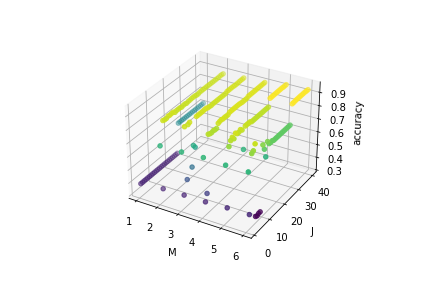
\includegraphics[width=0.8\textwidth]{/home/sathvikc/AMATH-482-2/AMATH-482/Homework Assignments/Homework 4/M_J_accuracyLotPoints.png}
    \caption{Plot of M and J values against accuracy for semi-supervised learning for a wide range of points}
    \label{fig:M_J_accuracy}
\end{figure}

We can see that our hypothesis is almost correct. There does seem to be wild drifts in the accuracy, 
but not as erratic as we saw in the spectral clustering case. Instead, these seem to be linked to a drop of directly 
correlated to the $J$ values. As $J$ increases by a factor of 10, it seems that accuracy increases as well. As such, this 
methodology does seem to be much more stable (no more rapid oscillation between varying accuracies). 

%This is perhaps the most important section of your report. You want to dedicate more space 
% here and present your numerical results in a clear, concise and meaningful way. Also 
% include a discussion of your numerics. Think hard about how you can use 
% your space most efficiently. For example, include subplots and multiple error curves on the 
% same plot etc. Ask us for advice when the time comes. 

% You will most definitely need tables and figures. So here is an example. 

% \begin{table}[htp]
%     \centering
%     \begin{tabular}{| l | c|c | r |}
%          \hline
%          row 1 & column 1  & column 2  \\ \hline
%          row 2 & column 1 & column 2 \\ 
%          row 3 & column 1 & column 2 \\ \hline
%     \end{tabular}
%     \caption{Don't forget to include a caption for your table. Say a few words about what is 
%     being shown.}
%     \label{tab:meaningful-label}
% \end{table}

% Make sure your table is labeled and referenced withing the text using $\backslash$\texttt{ref} as such Table~\ref{tab:meaningful-label}. In fact, you can 
% use $\backslash$\texttt{ref} to cite anything else in the document such as 
% sections (ex. Section~\ref{sec:Introduction}). This will create hyperlinks in your 
% pdf after compilation and automatically update the numbers and tags whenever you change 
% anything. 

% Figures are very similar to tables. Here's an example: 

% % \begin{figure}[htp]
% %     \centering
% %     \includegraphics[width=0.4\textwidth]{./Figs/fig1.pdf}
% %     \caption{Include a descriptive caption for your figure. Also make sure all 
% %     legends, axis labels, and titles are large enough to be readable. You might have 
% %     to reproduce the plots from Python or MATLAB with larger fonts for this purpose. It 
% %     can be annoying the first time you do it but it is crucial.}
% %     \label{fig:meaningful-label}
% % \end{figure}

% You may also need to include multiple figures: 

% % \begin{figure}
% %     \centering
% %     \begin{subfigure}[b]{.3\textwidth}
% %     \includegraphics[width=\textwidth]{./Figs/fig1.pdf}
% %     \caption{First subfigure}
% %     \label{subfig:first}
% %     \end{subfigure}
% %     \begin{subfigure}[b]{.3\textwidth}
% %     \includegraphics[width=\textwidth]{./Figs/fig2.pdf}
% %     \caption{First subfigure}
% %     \label{subfig:second}
% %     \end{subfigure}
% %     \begin{subfigure}[b]{.3\textwidth}
% %     \includegraphics[width=\textwidth]{./Figs/fig3.pdf}
% %     \caption{First subfigure}
% %     \label{subfig:third}
% %     \end{subfigure}
% %     \caption{Caption for entire figure. You don't need to use captions for subfigs so 
% %     feel free to eliminate the subcaption texts to just have the A, B, C labels.}
% %     \label{fig:meaningful-label-2}
% % \end{figure}

% Once again, make sure all your figures are referenced like Figure~\ref{fig:meaningful-label}
% or Figure~\ref{subfig:first} in the text body of the report and discussed 
% in detail. This is where you will make observations about your results and we will 
% look at these very closely. 

% Also note, I am using PDF figures. These give you the best looking graphs but PNG works 
% well too. I advise staying away from JPG as it always looks weird and low quality.]
% Both Python and MATLAB can output figures in PDF or PNG.

\section{Summary and Conclusions}\label{sec:conclusions}

% Wrap up your report with a brief summary of what you did and what you discovered. 
% Finish with some conclusions and possibly future directions if any. 

\section*{Acknowledgements}

% Make sure you you clearly state any help you received including collaborations 
% with your peers. Help from TAs or other mentors, professors, etc that helped you 
% with your assignment. Here's a formal example: 

% The author is thankful to Prof. X for useful discussions about the QR algorithm. 
% We are also thankful to Dr. Strange for suggesting the JAX software package for 
% automatic differentiation. Furthermore, our peer Jean Grey was helpful in 
% implementation of spectral clustering in Python.

 % make sure this matches the .bib file for your corresponding document. You also have to maintain your references in the .bib file 
\end{document}
